% CHAPTER SLIDE
\cscschapter{Scaling Up : Thread Blocks}

%%%%%%%%%%%%%%%%%%%%%%%%%%%%%%%%%%%%%%%%%%%%
\begin{frame}[fragile]{}
%%%%%%%%%%%%%%%%%%%%%%%%%%%%%%%%%%%%%%%%%%%%
    \begin{info}{}
        In the \axpy exercises we were limitted to 1024 threads for a kernel launch
        \begin{itemize}
            \item but we need to scale beyond 1024 threads for the \emph{massive parallelism} we were promised!
        \end{itemize}
    \end{info}

    \begin{info}{Thread blocks and grids}
        kernels are executed in groups of threads called \emph{thread blocks}
        \vspace{-12pt}
        \begin{itemize}
            \item the launch configuration \lst{axpy@<<<@grid_dim, block_dim@>>>@(...)}
            \begin{itemize}
                \item launch a \emph{grid} of \lst{grid_dim} \emph{blocks}
                \item each \emph{block} has \lst{block_dim} \emph{threads}
                \item for a total of \lst{grid_dim}$\times$\lst{block_dim} threads
            \end{itemize}
            \item previously we launched just one thread block \lst{axpy<<1, n>>(...)}
        \end{itemize}
    \end{info}

\end{frame}

%%%%%%%%%%%%%%%%%%%%%%%%%%%%%%%%%%%%%%%%%%%%
\begin{frame}[fragile]{}
%%%%%%%%%%%%%%%%%%%%%%%%%%%%%%%%%%%%%%%%%%%%
    \begin{info}{Why the additional complexity of grids+blocks+threads?}
        Because coordination and sharing between threads doesn't scale:
        \begin{itemize}
            \item threads in a block can synchronize and share resources
            \item this does not scale past a certain number of cores/threads
            \item on the K20X GPU streaming multiprocessor (SMX) has 192 CUDA cores, and can run 2028 threads
            \item threads in a block run on the same SMX, with shared resources and thread cooperation
            \item work is broken into blocks, which are distributed over the 14 SMXs in the K20X GPU
        \end{itemize}
    \end{info}
\end{frame}

%%%%%%%%%%%%%%%%%%%%%%%%%%%%%%%%%%%%%%%%%%%%
\begin{frame}[fragile]{}
%%%%%%%%%%%%%%%%%%%%%%%%%%%%%%%%%%%%%%%%%%%%
\begin{center}
\vspace{-0.75cm}
\begin{tabular}{|c|m{4cm}|m{5cm}|}
    \cline{1-2}
        concept & hardware &  \multicolumn{1}{c}{} \\
    \hline
        thread &
        \begin{minipage}{4cm}
            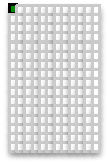
\includegraphics[width=0.3\textwidth]{./images/core.pdf}
        \end{minipage} &
        \footnotesize
        \begin{itemize}
            \item each thread executed on one core
        \end{itemize} \\
    \hline
        block &
        \begin{minipage}{4cm}
            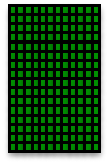
\includegraphics[width=0.3\textwidth]{./images/smx.pdf}
        \end{minipage} &
        \footnotesize
        \begin{itemize}
            \item block executed on 1 SMX
            \item multiple blocks per SMX if sufficient resources
            \item threads in a block share SMX resources
        \end{itemize} \\
    \hline
        grid &
        \begin{minipage}{4cm}
            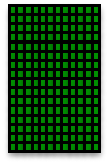
\includegraphics[width=0.3\textwidth]{./images/smx.pdf}
            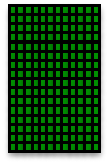
\includegraphics[width=0.3\textwidth]{./images/smx.pdf}
            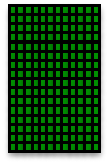
\includegraphics[width=0.3\textwidth]{./images/smx.pdf}
        \end{minipage} &
        \footnotesize
        \begin{itemize}
            \item kernel is executed in grid of blocks
            \item blocks distributed over SMXs
            \item multiple kernels can run at same time
        \end{itemize} \\
\hline
\end{tabular}
\end{center}
\end{frame}

%%%%%%%%%%%%%%%%%%%%%%%%%%%%%%%%%%%%%%%%%%%%
\begin{frame}[fragile]{}
%%%%%%%%%%%%%%%%%%%%%%%%%%%%%%%%%%%%%%%%%%%%
    \begin{info}{Calculating thread indexes}
        A kernel has to calculate the index of its work item
        \begin{itemize}
            \item in \lst{axpy} we used \lst{threadIdx.x} for the index
            \item when using multiple blocks, we need more information, which is available in the following \emph{magic variables}:
        \end{itemize}

        \begin{center}
            \begin{tabular}{ll}
            \lst{gridDim}   &: total number of blocks in the grid \\
            \lst{blockDim}  &: number of threads in a thread block \\
            \lst{blockIdx}  &: index of block \lst{[0, gridDim-1]} \\
            \lst{threadIdx} &: index of thread in thread block \lst{[0, blockDim-1]} \\
            \end{tabular}
        \end{center}

    \end{info}
\end{frame}

%%%%%%%%%%%%%%%%%%%%%%%%%%%%%%%%%%%%%%%%%%%%
\begin{frame}[fragile]{}
%%%%%%%%%%%%%%%%%%%%%%%%%%%%%%%%%%%%%%%%%%%%
    \begin{info}{Calculating thread indexes}
        Consider accessing an array of length 24 with 8 threads per block. The \emph{dimensions} of the kernel launch are:
        \begin{itemize}
            \item \lst{blockDim.x == 8} (8 threads/block)
            \item \lst{gridDim.x == 3} (3 blocks)
        \end{itemize}
        We calculate the index for our thread using the formula
        \begin{center}
            \lst{auto index = threadIdx.x + blockIdx.x*blockDim.x}\\
            \vspace{0.5cm}
            \centering 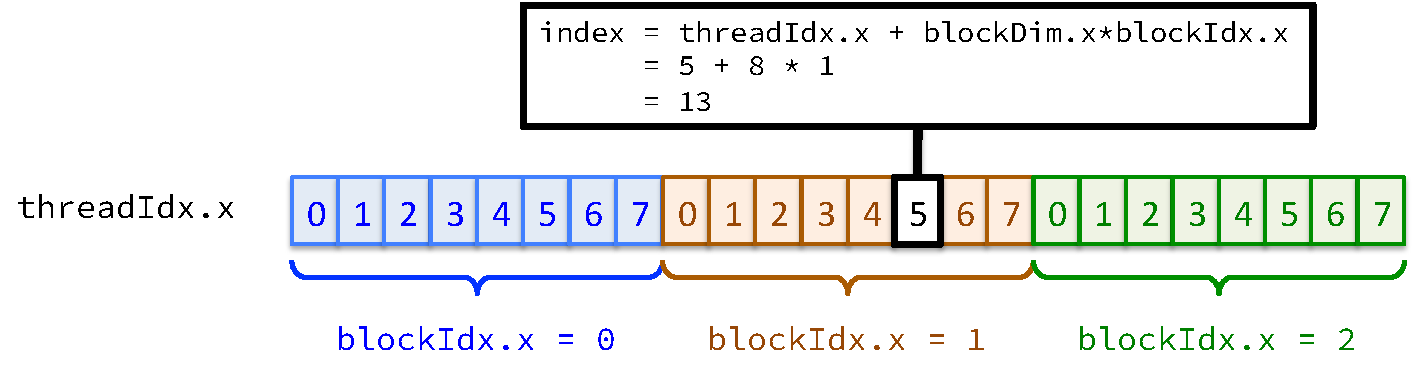
\includegraphics[width=\textwidth]{./images/blocks.pdf}
        \end{center}
    \end{info}
\end{frame}

%%%%%%%%%%%%%%%%%%%%%%%%%%%%%%%%%%%%%%%%%%%%
\begin{frame}[fragile]{}
%%%%%%%%%%%%%%%%%%%%%%%%%%%%%%%%%%%%%%%%%%%%
    \begin{info}{Calculating grid dimensions}
            The number of thread blocks and the number of threads per block are parameters for the kernel launch:
            \begin{center}
                \lst{kernel@<<<@blocks, threads_per_block@>>>@(...)}
            \end{center}
            Remember to guard against overflow when the number of work items is not divisible by the thread block size
    \end{info}

    \begin{code}{vector addition with multiple blocks}
%..................................
        \begin{lstlisting}[style=boxcudatiny]
__global__
void add_gpu(int *a, int *b, int n){
  auto i = threadIdx.x + blockIdx.x*blockDim.x;
  if(i<n) { // guard against access off end of arrays
    a[i] += b[i];
  }
}

// in main()
auto block_size = 512;
auto num_blocks = (n + (block_size-1)) / block_size;
add_gpu@<<<@num_blocks, block_size@>>>@(a, b, n);
        \end{lstlisting}
%..................................
    \end{code}
\end{frame}

%%%%%%%%%%%%%%%%%%%%%%%%%%%%%%%%%%%%%%%%%%%%
\begin{frame}[fragile]{}
%%%%%%%%%%%%%%%%%%%%%%%%%%%%%%%%%%%%%%%%%%%%
    \begin{info}{Calculating grid dimensions}
        We have to take care when calculating the number of blocks in the grid, i.e. \lst{blocks}:
        \begin{center}
            \lst{kernel@<<<@blocks, threads_per_block@>>>@(...)}
        \end{center}
        Most likely, the number of work items \lst{n} is not a multiple of \lst{threads_per_block}.
        \begin{itemize}
            \item in this case we have one thread block in which not all threads will work
        \end{itemize}
    \end{info}

    \begin{code}{Calculating grid dimensions}
%..................................
        \begin{lstlisting}[style=boxcudatiny]
auto block_size = 512;
auto num_blocks = (n + (block_size-1)) / block_size;
add_gpu@<<<@num_blocks, block_size@>>>@(a, b, n);
        \end{lstlisting}
%..................................
    \end{code}
\end{frame}

%%%%%%%%%%%%%%%%%%%%%%%%%%%%%%%%%%%%%%%%%%%%
\begin{frame}[fragile]{}
%%%%%%%%%%%%%%%%%%%%%%%%%%%%%%%%%%%%%%%%%%%%
    \begin{info}{The number of threads per block impacts performance}
    \begin{itemize}
        \item the optimal number depends on the resources (registers, shared memory, etc) that a kernel requires
    \end{itemize}
    \end{info}

    \begin{code}{Choosing block size automatically (CUDA 6.5 and later)}
%..................................
        \begin{lstlisting}[style=boxcudatiny]
int block_size, min_grid_dim;

cudaOccupancyMaxPotentialBlockSize
  (&min_grid_size, &block_size, add_gpu, 0, n);
auto num_blocks = (n + (block_size-1)) / block_size;

add_gpu@<<<@num_blocks, block_size@>>>@(a, b, n);
        \end{lstlisting}
%..................................
    \end{code}

    \begin{info}{}
    The variable \lst{min_grid_size} is set to the minimum number of blocks required to \emph{saturate} the GPU, i.e. provide the GPU with enough work to utilize all of the SMXs.
    \end{info}
\end{frame}

%%%%%%%%%%%%%%%%%%%%%%%%%%%%%%%%%%%%%%%%%%%%
\begin{frame}[fragile]{Exercise: Blocks}
%%%%%%%%%%%%%%%%%%%%%%%%%%%%%%%%%%%%%%%%%%%%
    Open \lst{cuda/exercises/axpy.cu} from the last exercise
    \begin{enumerate}
        \item Extend the \axpy kernel for arbitrarily large input arrays (any \lst{n})

        \item Update the call site to calculate the grid configuration

        \item Compile the test and run
        \begin{itemize}
            \item it will pass with no errors on success
        \end{itemize}

        \item Experiment with varying the size of the arrays (scaling)
        \begin{itemize}
            \item start small and increase
            \item how does it affect the kernel execution time?
        \end{itemize}

        \item \extra Compare scaling with the \lst{axpy_omp} benchmark

        \item \extra Experiment with varying the block size
        \begin{itemize}
            \item try \lst{block_size} calculated by \lst{cudaOccupancyMaxPotentialBlockSize}.
        \end{itemize}

    \end{enumerate}

\end{frame}

%%%%%%%%%%%%%%%%%%%%%%%%%%%%%%%%%%%%%%%%%%%%
\begin{frame}[fragile]{Exercise: Results}
%%%%%%%%%%%%%%%%%%%%%%%%%%%%%%%%%%%%%%%%%%%%

%\begin{tikzpicture}
%    \pgfplotsset{footnotesize}
%    \begin{semilogyaxis}[
%        height=0.7\textwidth,
%        width=\textwidth,
%        xmin=8,xmax=28,
%        xtick={8,12,16,20,24,28},
%        xlabel=$log_2(n)$,
%        ylabel=time (s),
%        legend style = {at={(0.05,0.95)}, anchor=north west},
%        every axis y label/.style=
%            {at={(ticklabel cs:0.5)},rotate=90,anchor=near ticklabel},
%        grid=major]
%        \addplot[color=blue,mark=*]  table[x=n,y=gpu]  {./plots/axpy.tbl};
%        \addplot[color=red,mark=*]   table[x=n,y=omp1] {./plots/axpy.tbl};
%        \addplot[color=green,mark=*] table[x=n,y=omp8] {./plots/axpy.tbl};
%        \legend{CUDA, OpenMP 1, OpenMP 8};
%    \end{semilogyaxis}
%\end{tikzpicture}

\begin{center}
\begin{tikzpicture}
    \pgfplotsset{footnotesize}
    \begin{axis}[
        height=0.4\textwidth,
        width=\textwidth,
        xmin=8,xmax=28,
        ymin=0,ymax=6,
        xtick={8,12,16,20,24,28},
        ytick={0,1,2,3,4,5,6},
        xlabel=$log_2(n)$,
        ylabel=speedup,
        legend style = {at={(0.05,0.95)}, anchor=north west},
        every axis y label/.style=
            {at={(ticklabel cs:0.5)},rotate=90,anchor=near ticklabel},
        grid=major]
        \addplot[color=blue,mark=*]  table[x=n,y expr=\thisrow{omp8}/\thisrow{gpu}]  {./plots/axpy.tbl};
        \addplot[color=black,mark=*] table[x=n,y expr=\thisrow{omp8}/\thisrow{omp8}] {./plots/axpy.tbl};
        \legend{CUDA speedup, OpenMP 8 thread};
    \end{axis}
\end{tikzpicture}
\end{center}

The GPU is a throughput device:
\begin{itemize}
\item the CUDA implementation is faster for $2^{15}\approx32,000$
\item requires $2^{20}\approx1,000,000$ to get ``advertised'' $5\times$ speedup
\end{itemize}
You have to provide enough parallelism to exploit many cores

\end{frame}

% cudaOccupancyMaxPotentialBlockSize suggests block_dim 256-1024, depending on n
% in practice it makes little difference

